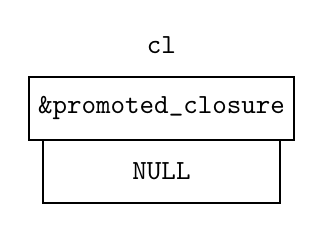
\begin{tikzpicture}[
blank/.style={node distance=0.8cm, font=\ttfamily},
block/.style={rectangle, text centered, thick, draw=black, font=\ttfamily,
minimum width=3cm, minimum height=0.8cm, node distance=0.8cm},
block-header/.style={block, node distance=6cm},
block-body/.style={block}
]

\node [block-header] (f) {\verb|&promoted_closure|};
\node [blank, above of=f] (cl-f) {cl};
\node [block-body, below of=f] (f-next) {NULL};

\end{tikzpicture}